% Contains placeholder stuff

\chapter{Einleitung}
\label{chp:Einleitung}
Lorem ipsum dolor sit amet, consectetuer adipiscing elit, sed diam nonummy nibh euismod tincidunt ut laoreet dolore magna aliquam erat volutpat. Ut wisi enim ad minim veniam, quis nostrud exerci tation ullamcorper suscipit lobortis nisl ut aliquip ex ea commodo consequat. \cite{Konak2006,Sailer2013}

Lorem ipsum dolor sit amet, consectetuer adipiscing elit, sed diam nonummy nibh euismod tincidunt ut laoreet dolore magna aliquam erat volutpat. Ut wisi enim ad minim veniam, quis nostrud exerci tation ullamcorper suscipit lobortis nisl ut aliquip ex ea commodo consequat.
 
 
 \chapter{Hauptteil}
 \label{sec:Hauptteil}
 
 Abbildungen k\"{o}nnen im Unterverzeichnis \texttt{figures} abgelegt werden.
 Eingebunden werden Sie mit dem Befehl \texttt{\textbackslash includegraphics} innerhalb
 einer \texttt{figure}-Umgebung:
 \begin{figure}[htb]
 	\centering
 	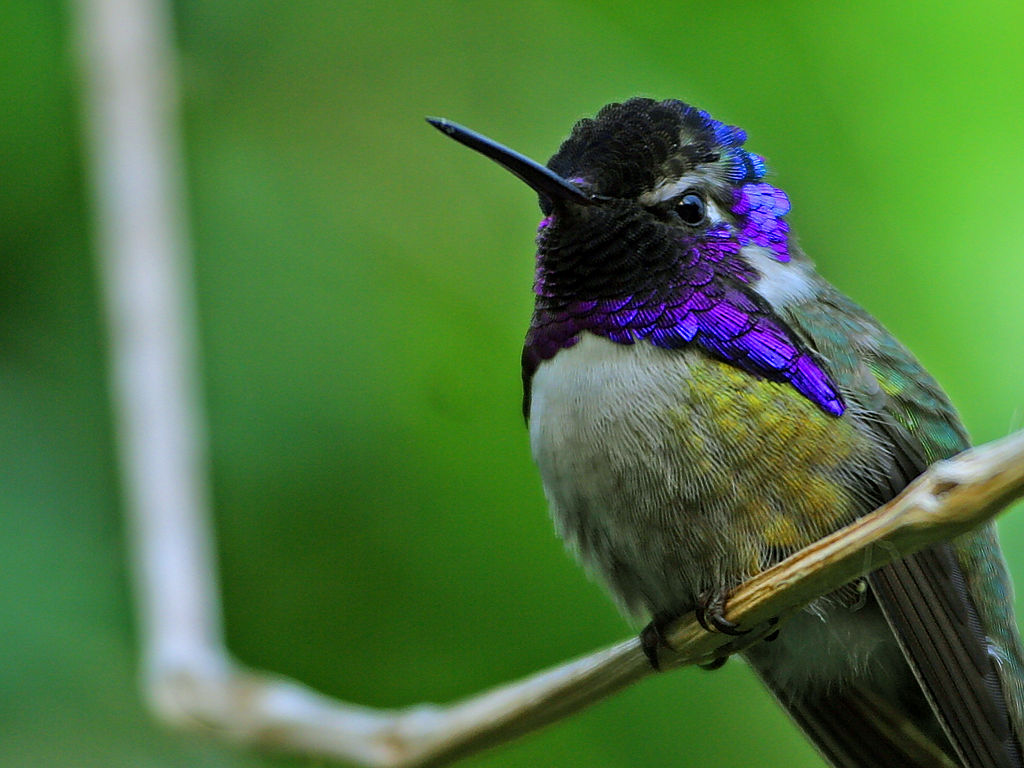
\includegraphics[width=0.8\textwidth]{figures/Hummingbird.jpg}
 	\caption{Eine Veilchenkopfelfe (auch Costakolibri genannt, vom lateinischen Calypte costae), die zur Familie der Kolibris geh\"{o}rt \cite{Kolibri}}
 	\label{fig:kolibri}
 \end{figure}
 
 \section{Erste Zwischen\"{u}berschrift}
 \label{sec:ErsteZwischenueberschrift}
 Die Arbeit kann auch Tabellen im \texttt{table}-Environment enthalten:
 \begin{table}[ht]
 	\centering
 	\caption{Entfernungstabelle S\"{u}ddeutschland, vgl. \cite{entfernungstabelle}}
 	\begin{tabular}{c r r r}
 		\toprule
 		& Augsburg & M\"{u}nchen & Stuttgart \\
 		\midrule
 		Augsburg  & -        & 61      & 149       \\
 		M\"{u}nchen   & 61       & -       & 210       \\
 		Stuttgart & 149      & 210     & -         \\
 		\bottomrule
 	\end{tabular}
 	\label{tab:entfernungen}
 \end{table}
 
 \subsection{Erste Unter\"{u}berschrift}
 \label{sec:ErsteUnterueberschrift}
 
 Das \texttt{listings}-Paket erlaubt es, Quellcode mit Syntax-Highlighting einzubinden:
 
 \begin{lstlisting}[language=Python,float=ht,caption={Python-Programm zur Berechnung der Fakult\"{a}tsfunktion}]
 def fact(n):
 """Return the n-th factorial number"""
 if n == 0:
 return 1
 else:
 return n * fact(n-1)
 
 # Test output
 print fact(10)
 print "Done"
 \end{lstlisting}
 \label{lst:factorial}  
 
 \section{Zweite Zwischen\"{u}berschrift}
 \label{sec:ZweiteZwischenueberschrift}
 
 TEXT
 
 \chapter{Schluss}
 \label{chp:Schluss}
 
 TEXT
 
 %%% Local Variables:
 %%% mode: latex
 %%% TeX-master: "../Abschlussarbeit"
 %%% End:
 